\chapter{Shamir 秘密共享}

\section{实验目的}

巩固对Shamir秘密共享算法的理解。

\section{实验要求}

实现一个(k,n)-Shamir 秘密共享方案,其中k=3,n=5,包含以下功能:
\begin{enumerate}
    \item 给定一个数字,可以计算出对应的share
    \item 给定k个share, 能够重构出秘密值。
\end{enumerate}

\section{实验内容}

\subsection{Shamir 秘密共享算法分析}

Shamir的秘密共享方案是由Adi Shamir提出的最早的秘密共享算法,
它的实现基于有限域上多项式的插值\cite{contributors_2019}。

此处我们不加证明的给出Langrange插值定理。

\begin{theorem}
    \label{the:lang}
    给定$n$个互异点$P_i=(x_i,y_i)\in \mathbb{F}^2,\forall x_i \neq x_j, i \neq j,0\leq i,j < n$,
    则可唯一确定$n-1$阶多项式$f(x)\in \mathbb{F}[x]$,且有:
    \begin{equation*}
        f(x) = \sum_{i=1}^{n} y_i \left(
            \prod_{j\neq i}^{1\leq j \leq n}\frac{x-x_j}{x_i-x_j}
        \right)
    \end{equation*}
\end{theorem}

根据秘密共享的要求,给定$(k,n)$秘密共享方案,则需要被共享的数据
被分为$n$份share,其中任意$k$或多于$k$份share都能还原本来的数据,
而任意少于$k$份share都不包含原来数据的任何信息。

因此,我们可以这样设计基于多项式插值的秘密共享方案:
\begin{enumerate}
    \item \textbf{多项式准备}:以常数项为数据,随机生成有限域$\mathbb{F}$上的多项式$f(x)$;
    \item \textbf{数据分割}:生成多项式$f(x)$上的$n$个互异点,将其坐标信息打包为share;
    \item \textbf{数据重构}:利用$k$个share中的坐标信息进行多项式插值,重构原来的多项式$f(x)$,取其常数项$f(0)$即为还原的数据。
\end{enumerate}

\newpage
\subsection{程序设计与实现}

    具体代码见附录\ref{appendix:Shamir},此处仅对关键设计进行说明。

\subsubsection{Element类设计}

根据上文可以知道,所给的插值方法是在有限域上进行的,因此笔者设计了Element类
来封装有限域$\mathrm{GF}(2^{128})$上的元素运算。

其中设置有限域为$\mathrm{GF}(2^{128})$的原因是,它可以表示128bit的信息,
而目前的AES加密算法的密钥长度最小即为128bit,因此该方案在实现后可以用于
对AES密钥的共享。而在需要共享数据时,就可先用AES对其进行加密,并把密文放置在
公共空间中,通过分发AES密钥的share来缩短share长度,并实现相同效果。

此外,该类重构了乘法,加法和幂次运算,并且基于扩展欧几里得算法设计了求模逆元的方法。
具体在求模数时,查表得到$\mathrm{GF}(2^{128})$的一个本原多项式
$1+x+x^2+x^7+x^{128}$,
即可取模数irr\_poly为$1 + 2 + 4 + 128 + 2 ^ {128}$。

\subsubsection{Shamir类设计}

Shamir类包含了split和combine两个静态方法。

\textbf{数据分割}:split方法即为数据分割,要求传入方案参数$k, n$以及要分割的数据secret。
在多项式准备过程中,通过Crypto库的Random类生成伪随机数(保证其为PRG生成),
将常数项设置为分割数据secret。

取点过程中直接取$x_i = 1, 2, \cdots, n, 0\leq i < n$,通过迭代运算得到$y_i$。
最后打包为Python中的列表对象返回shares。

\textbf{数据重构}:combine方法即为数据重构,要求传入shares。不要求给定
原来的方案参数,因为当shares的数目$m<k$时,插值得到多项式错乱,无需要信息,
而$m>k$时,由于点$P_k, P_{k+1}, \cdots, P_m$仍在前$k$个点还原的多项式上,
因此最后的插值结果不会发生改变。

具体在计算中即利用了定理\ref{the:lang}中的公式,不再说明。

\newpage
\subsubsection{图形化界面设计}

如下图\ref{fig:shamir}所示即为设计的3,5-Shamir秘密共享方案图形化界面,
设计用到Python的PyQt5库。

\begin{figure}[!htbp]
    \centering
    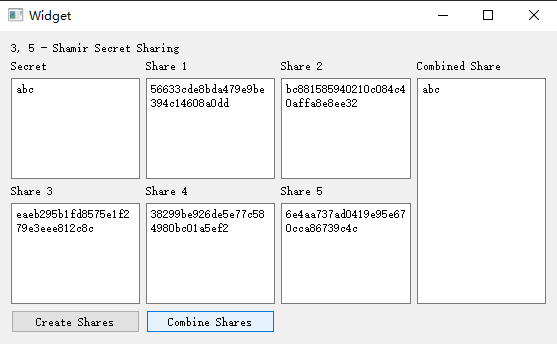
\includegraphics[width=0.7\textwidth]{figures/shamir.png}
    \caption{3,5-Shamir秘密共享方案的图形化界面}
    \label{fig:shamir}
\end{figure}

给定文本框Secret中的内容,点击Create Shares即可获得5份share
(share通过binascii库的hexlify函数转化为16进制格式),或者输入
5份share后,点击Combine Shares即可在文本框Combined Share显示原来的数据内容。

其中,combine过程的share选择取决于文本框Share 1-5是否有内容,如有则会提取。
由于选定门限为3,5,因此3份或以上的share可以还原,少于3份则会显示为NULL,如下图\ref{fig:shamir_2}所示。

\begin{figure}[!htbp]
    \centering
    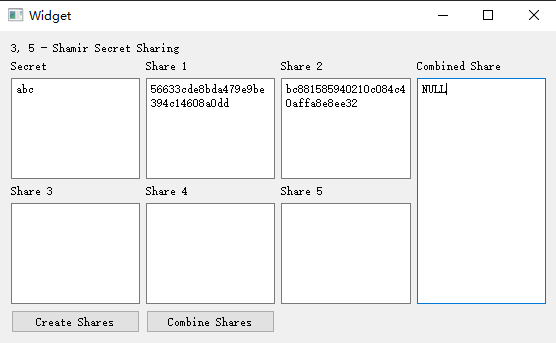
\includegraphics[width=0.7\textwidth]{figures/shamir_2.png}
    \caption{3,5-Shamir秘密共享方案恢复失败的结果}
    \label{fig:shamir_2}
\end{figure}

\subsection{图像秘密共享方案的讨论}

该处给出了一种基于上文所给的Shamir秘密共享的图像秘密共享方案。
我们知道图像在计算机存储时可认为是二维矩阵的存储,因此只需要将
矩阵中的每一个元素进行秘密共享,即可对原本的图像进行共享。
最终结果如图\ref{fig:shamir_3}所示。

\begin{figure}[!htbp]
    \centering
    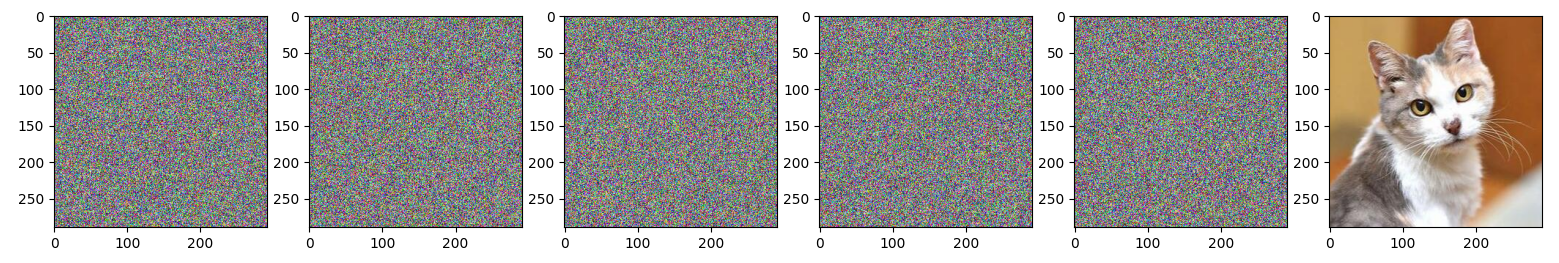
\includegraphics[width=1\textwidth]{figures/shamir_3.png}
    \caption{3,5-图像秘密共享方案的结果}
    \label{fig:shamir_3}
\end{figure}

可看到图\ref{fig:shamir_3}中前五张图即为原本的秘密共享结果,图像和噪点图类似。
任取前5张图中的3张以上图片即可还原出第六张图片。

对于一张$n\times n$像素的彩图,需要进行$4n^2$次秘密共享,因此该方法的效率
还是较低的。从改进角度考虑,可将原本的有限域取为$\mathrm{GF}(2^8)$即可
完成RGB图像编码的数值范围要求,从而降低生成多项式的阶数来提高效率。

此外由于产生的图像类似于噪点图,可作为滤镜作用于其他图像上,最后通过提取算法
即可进行share的隐秘化。